% 第1章 システムアーキテクチャ
\section{システムアーキテクチャ}
\subsection{BIOS}
\begin{description}
	\item[入出力基本システム(BIOS : Basic Input Output System)]\mbox{}\\
	コンピュータに接続されたディスクドライブ、キーボード、ビデオカードなどの周辺機器を制御するプログラム群のこと.
		\begin{itemize}
			\item{OSを起動するためのプログラムをディスクから読み込んで実行}
			\item{デバイスの動作を設定}
			\item{基本的な入出力を制御する}
		\end{itemize}
\end{description}

\subsection{デバイス}
\subsubsection{デバイス確認}
Linuxカーネルが認識しているデバイスは/proc以下で確認が可能(図\ref{001}).
\begin{figure}[!h]
	\begin{center}
		\includegraphics[width=10cm]{./section1/pic/001.eps}
		\caption{/procの内容}
		\label{001}
	\end{center}
\end{figure}

\begin{table}[htb]
  \begin{center}
    \begin{tabular}{|l|l|} \hline
      ファイル名 & 情報 \\ \hline
      cpuinfo & CPU情報 \\ \hline
      meminfo & メモリ情報 \\ \hline
      net & ネットワーク情報 \\ \hline
      mounts & マウントされたデバイス情報 \\ \hline
      partitions & パーティション情報 \\ \hline
      bus & bus情報 \\ \hline
    \end{tabular}
    \caption{/procのファイル例}
  \end{center}
\end{table}

Linuxはハードウェアへのアクセスを抽象化するデバイスファイルを持っており,これのデバイスファイルの読み書きを通してハードウェアにアクセスする.
このとき,/devディレクトリに接続されているデバイスが認識されていなければ利用できない(図\ref{002}).

\begin{figure}[!h]
	\begin{center}
		\includegraphics[width=10cm]{./section1/pic/002.eps}
		\caption{/devの内容}
		\label{002}
	\end{center}
\end{figure}

デバイスを確認するためのコマンドも用意されている.

\begin{table}[htb]
  \begin{center}
    \begin{tabular}{|l|l|} \hline
      コマンド名 & 情報 \\ \hline
      lspci & PCIデバイス情報(図\ref{003}) \\ \hline
      lsusb & USBデバイス情報(図\ref{004}) \\ \hline
      dmidecode & DMI情報(図\ref{005}) \\ \hline
      fdesk -l & ディスクの空き容量情報 \\ \hline
      free -m & メモリの空き容量情報 \\ \hline
      bus & bus情報 \\ \hline
    \end{tabular}
    \caption{デバイス情報を確認できるコマンド例}
  \end{center}
\end{table}

\begin{figure}[!h]
	\begin{center}
		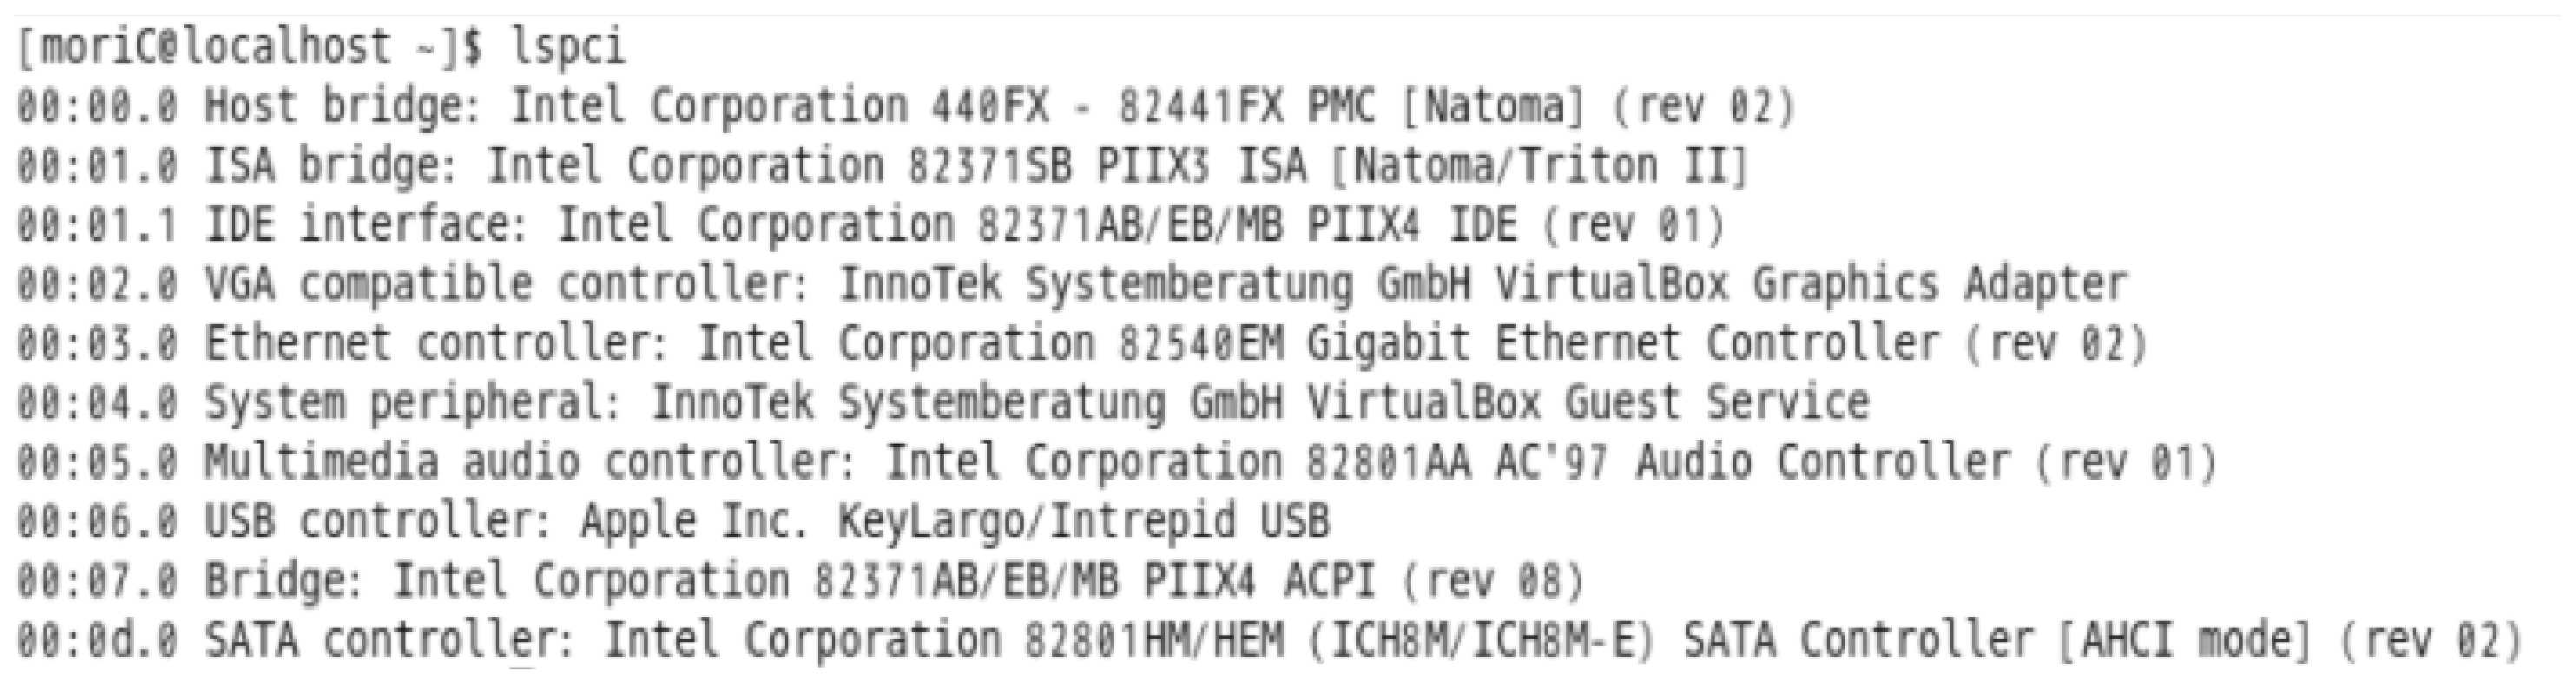
\includegraphics[width=10cm]{./section1/pic/003.eps}
		\caption{lspciの内容}
		\label{003}
	\end{center}
\end{figure}

\begin{figure}[!h]
	\begin{center}
		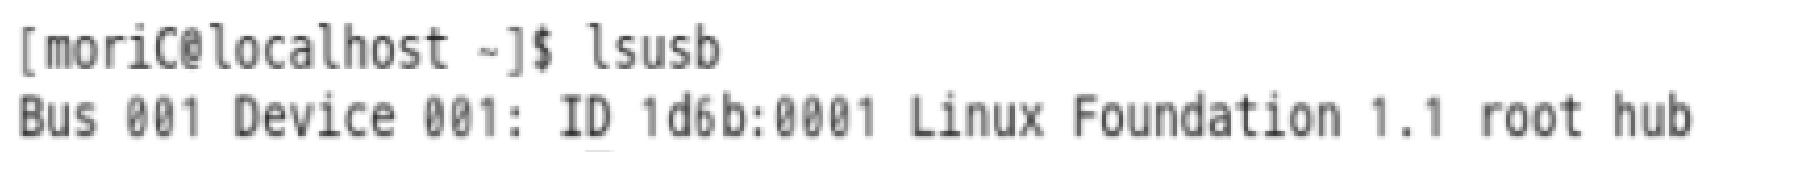
\includegraphics[width=10cm]{./section1/pic/004.eps}
		\caption{lsusbの内容}
		\label{004}
	\end{center}
\end{figure}

\begin{figure}[!h]
	\begin{center}
		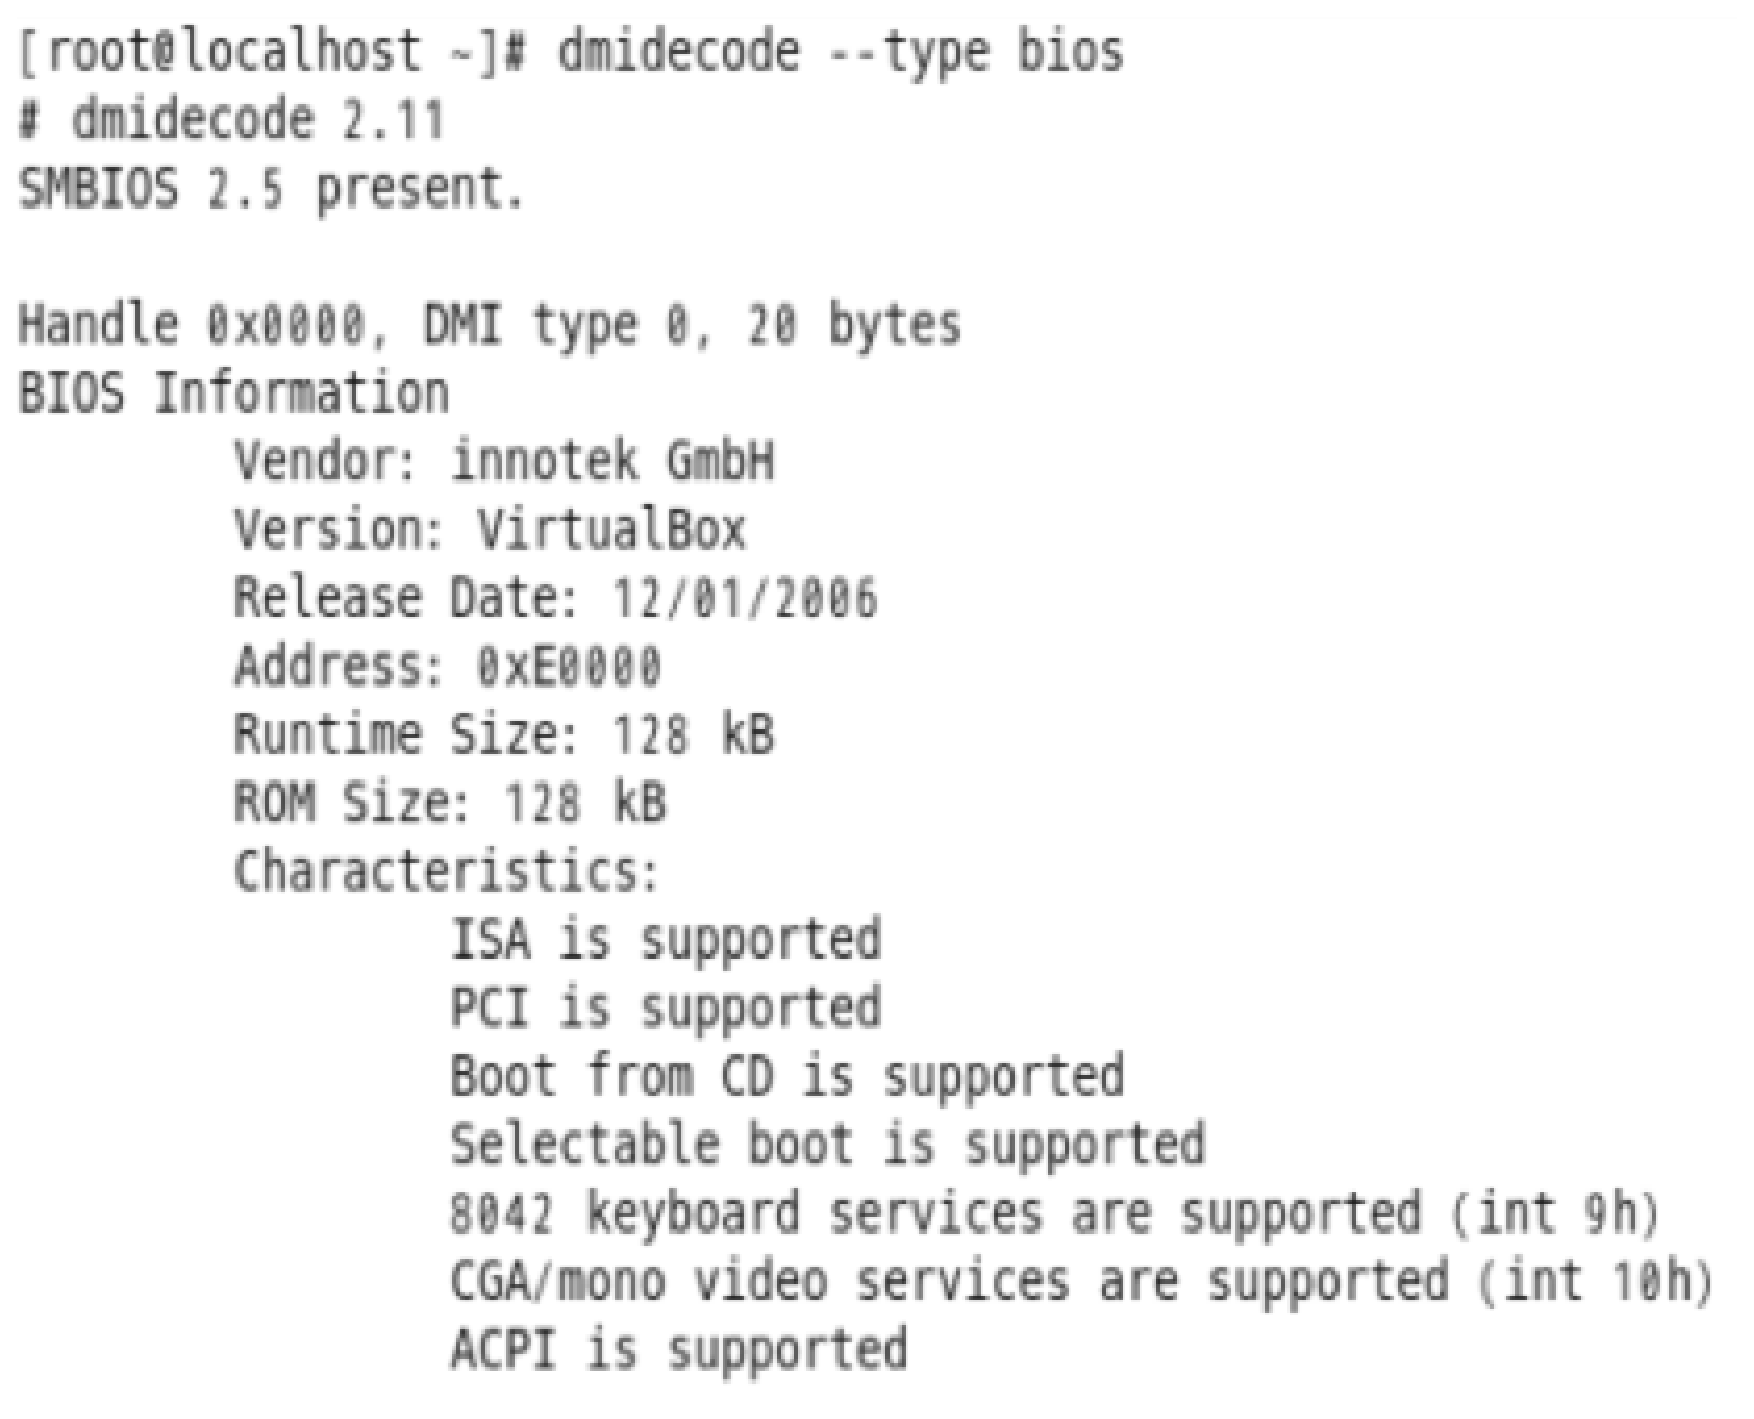
\includegraphics[width=10cm]{./section1/pic/005.eps}
		\caption{dmidecodeの内容}
		\label{005}
	\end{center}
\end{figure}

\clearpage
\subsubsection{デバイスドライバロード}
\begin{description}
	\item[デバイスドライバ(device driver)]\mbox{}\\
	デバイスを利用するために必要な制御プログラムで必要なデバイスドライバを取り込むことを「ロードする」という.
	基本的には自動的にロードされる.
	\item[lsmod]\mbox{}\\
	ロードされているカーネルモジュールを確認するコマンド(図\ref{006})
		\begin{figure}[!h]
			\begin{center}
				\includegraphics[width=10cm]{./section1/pic/006.eps}
				\caption{lsmodの内容}
				\label{006}
			\end{center}
		\end{figure}
	\item[modprobe]\mbox{}\\
	手動でデバイスドライバをロードするコマンド
\end{description}


\clearpage
\subsection{システムの起動}
\subsubsection{システム起動の流れ}
\begin{figure}[!h]
	\begin{center}
		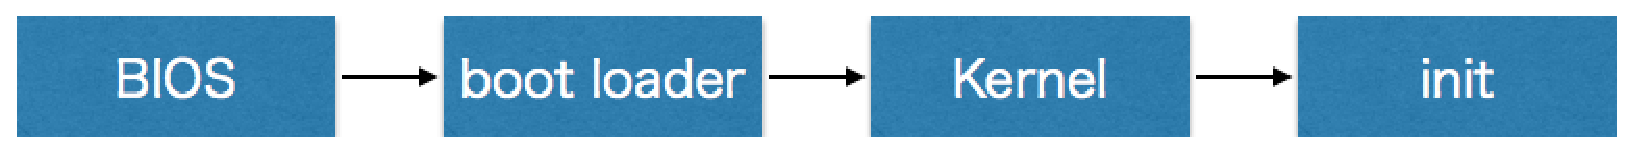
\includegraphics[width=10cm]{./section1/pic/007.eps}
		\caption{システム起動の流れ}
		\label{007}
	\end{center}
\end{figure}
\begin{enumerate}
	\item BIOSではハードウェアのチェックや初期化を実行し,ディスクのブートセクタを読み出しブートローダへ制御を移す.
	\item ブートローダでは	ハードディスクからカネールをメモリへ読み込む.
	\item カーネルではメモリの初期化やシステムクロックの設定を実行し,initプログラム実行へ移す.
	\item initプログラムでは初期化スクリプトを実行してランレベルに応じて指定したデーモンを起動する.
\end{enumerate}

\subsubsection{システム起動時イベント}
\begin{description}
	\item[dmesg]\mbox{}\\
	システム起動時の処理を確認できるコマンド.カーネルが出力したメッセージを一時的に蓄えておくバッファの内容を表示する./var/log/messageのログファイルにシステム起動時の状況が保存されている.(図\ref{008})
		\begin{figure}[!h]
			\begin{center}
				\includegraphics[width=10cm]{./section1/pic/008.eps}
				\caption{dmesgの内容(抜粋)}
				\label{008}
			\end{center}
		\end{figure}
\end{description}

\subsubsection{initプロセス}
\begin{description}
	\item[initプロセス]\mbox{}\\
	Linuxシステムで最初に実行されるプロセスで,/etc/inittabファイル(図\ref{009})の設定を読み込み,システムに必要なサービスを順次起動していく.一般的なUNIX系OSではSysVinitが実行される.
		\begin{figure}[!h]
			\begin{center}
				\includegraphics[width=10cm]{./section1/pic/009.eps}
				\caption{inittabの内容}
				\label{009}
			\end{center}
		\end{figure}
\end{description}
\begin{description}
	\item[SysVinit]\mbox{}\\
 SystemV initの略.UNIX SystemVで採用された起動の仕組み.あらかじめ決められた順位サービスを起動していくため,サービスの起動時間によって全体の起動時間が変動する.
		\begin{enumerate}
			\item /etc/inittabファイルを読み込む.
			\item /etc/rc.sysinitスクリプトを実行.
			\item /etc/rcスクリプトを実行.
			\item /etc/rcスクリプトが/etc/rc(ランレベル).dディレクトリ以下のスクリプトを実行.
		\end{enumerate}
	\item[Upstart]\mbox{}\\
 イベント駆動型のinitデーモンで,ブート時のタスクの起動とシャットダウン時のタスクの停止を非同期に行い、同時にシステム動作中の管理を行う.
	\item[systemd]\mbox{}\\
 ソケット起動型サービスとバス起動型サービスを組み合わせたinitデーモンで,相互に依存したサービス群をより並列的に起動できる.
\end{description}

\subsection{ランレベル}